\documentclass{article}
\usepackage{imakeidx} % Per creare un vero indice
\usepackage{amsmath}
\usepackage{booktabs}
\usepackage{verbatim}
\usepackage{listings} %Python
\usepackage{amsfonts}
\usepackage{tcolorbox}
\usepackage{titlesec}
\usepackage[utf8]{inputenc}
\usepackage[italian]{babel}
\usepackage{ragged2e}
\usepackage{setspace}
\usepackage{caption}
\usepackage{fancyhdr}
\usepackage{listings}
\usepackage{algorithm}
\usepackage{algpseudocode}
\usepackage{hyperref}
\usepackage{tikz}
\usepackage{float}
\usepackage{array}
\usepackage{graphics}
\usepackage{multirow}
\usepackage{listings}
\usepackage{booktabs}
\usepackage{tabularx}
\usepackage{pythonhighlight}
\usetikzlibrary{arrows}
\usepackage{graphicx} % Importa il pacchetto graphicx per l'inserimento di immagini
\usepackage{multicol} % Per avere la multicolonna
\usepackage[a4paper, top=3cm, bottom=4cm, left=3cm, right=3cm, includehead, includefoot]{geometry}
% Imposta il carattere Times New Roman
\usepackage{mathptmx}
\usepackage{titlesec} % Per \HRule
\definecolor{main}{HTML}{5989cf}
\definecolor{sub}{HTML}{cde4ff} 
\newcommand{\HRule}{\rule{\linewidth}{0.5mm}}

\newtcolorbox{boxC}{
	colback = sub, % background color
	boxrule = 0pt  % no borders
}

\lstset{ 
	language=python, 
	basicstyle=\ttfamily\footnotesize,
	frame=single, 
	numbers=left, 
	numberstyle=\tiny\color{gray}, 
	stepnumber=1, 
	numbersep=5pt, 
	backgroundcolor=\color{white}, 
	showspaces=false, 
	showstringspaces=false, 
	showtabs=false, 
	frame=single, 
	rulecolor=\color{black}, 
	tabsize=4, 
	captionpos=b, 
	breaklines=true, 
	breakatwhitespace=true, 
	title=\lstname, 
	keywordstyle=\color{blue}, 
	commentstyle=\color{purple}, 
	stringstyle=\color{violet}, 
}
\renewcommand{\headrulewidth}{0pt}
\setlength{\headheight}{60pt} % Altezza dell'intestazione
\setlength{\headsep}{50pt} % Distanza intestazione - contenuto

\makeindex % Indice
\begin{document}
	
	\begin{titlepage}
		\thispagestyle{fancy} % Stile fancy solo per questa pagina
		\fancyhf{} % Cancella intestazioni e piè di pagina di default
		\fancyhead[L]{
\includegraphics[width=4.5cm]{immagini/logodisamis.jpg}} % Immagine a sinistra
		\fancyhead[R]{
\includegraphics[width=3cm]{immagini/logounisa.png}} % Immagine a destra
		\begin{center}
			
			% Topo
			\textsc{\LARGE Universit\`a degli Studi di Salerno}\\[1.5cm]
			\textsc{\large DIPARTIMENTO DI SCIENZE AZIENDALI - MANAGEMENT \& INNOVATION SYSTEMS}\\[0.2cm]
			\textsc{\large Corso di Laurea Magistrale in Data Science \& Gestione dell'Innovazione}\\[3.5cm]
			
			% Titolo
			{ \huge \bfseries Esame di Massive Data Mining}\\[0.4cm]
			{ \huge TMDB 5000 Movie Dataset Title Recommendation System}\\[0.4cm]

			
			\begin{center}
				\textbf{A.A. 2024-2025} \\ [2.50cm]
				\textbf{Docenti:} \\[0.2cm]
				\textbf{Domenico Parente} \\[0.2cm]
				\textbf{Luca Rizzuti} \\ [4.0cm]
				\textbf{\bfseries Candidata:\\}
				\textsc{Denise Brancaccio - Mat. 0222800163}\\

				
			\end{center}
			
		\end{center}
	\end{titlepage}
	\newpage
	
	\tableofcontents
	
	\newpage
	\section{Introduzione}
	La seguente documentazione illustra il progetto realizzato per l'esame di Massive Data Mining, incentrato sulla creazione di un motore di ricerca per il TMDB 5000 Movie Dataset, il quale raccoglie vaste informazioni su 5000 film diversi includendo:
	\begin{itemize}
	\item Title;
	\item Genres;
	\item Overview;
	\item Cast e Crew;
	\item Production Companies;
	\item Keywords;
	\item Ratings;
	\end{itemize}
	L'obiettivo \`e creare un sistema di raccomandazione sui film in grado di restituire, a partire da una query immessa dall'utente, i 10 film più pertinenti. La query può essere il titolo di un film, scritto in modo approssimativo o corretto, uno o più generi, una trama generale, il nome di un membro del cast o la compagnia di produzione. L'obiettivo principale del progetto \`e gestire in modo robusto situazioni reali, tenendo conto sia la possibilità che le query siano precise, sia che possano presentare imprecisioni come titoli parziali, errori di battitura, descrizioni molto generiche della trama.\\
	Per realizzare questo lavoro sono state utilizzati due approcci: la cosine similarity, realizzata tramite embedding vettoriali generati dal modello "all-MiniLM-L6-v2" della libreria SentenceTrasformers, e la FuzzySearch, metodo della libreria thefuzz basato sulla distanza di Levenshtein, a sua volta basata su quelle di Hamming e Manhattan, ed utilizzato per la ricerca in caso di titoli o nomi parziali. 
	
\subsection{Strumenti e Tecnologie Utilizzate}
	Al fine della realizzazione del progetto \`e stato utilizzato il linguaggio di programmazione Python tramite un Notebook Jupiter per ottimizzare la pulizia del codice. Sono inoltre state impiegate le seguenti librerie:
	\begin{itemize}
		\item \textbf{pandas}: utilizzata per la manipolazione e l'analisi dei dati tabellari tramite DataFrame.
		
		\item \textbf{ast}: impiegata per convertire rappresentazioni testuali di strutture dati Python (es. liste o dizionari) in oggetti utilizzabili dal programma.
		
		\item \textbf{numpy}: utilizzata per operazioni numeriche efficienti su array e matrici.
		
		\item \textbf{thefuzz}: libreria per il \textit{fuzzy matching}, impiegata per misurare la somiglianza tra stringhe anche in presenza di errori o variazioni testuali.
		
		\item \textbf{sentence-transformers}: utilizzata per generare embedding semantici di frasi e testi mediante modelli basati su Transformer.
		
		\item \textbf{scikit-learn} (\texttt{cosine\_similarity}): utilizzata per calcolare la similarità coseno tra vettori, ad esempio tra embedding testuali.
	\end{itemize}
	Inoltre per le realizzazione dell'Analisi Esplorativa dei Dati, sono state utilizzate anche le librerie:
	\begin{itemize}
		\item \textbf{seaborn}: libreria per la visualizzazione statistica dei dati, utilizzata per creare grafici informativi e facilmente interpretabili.
		
		\item \textbf{plotly.express}: modulo di Plotly che consente di generare grafici interattivi in modo semplice e rapido.
		
		\item \textbf{collections} (\texttt{Counter}): struttura dati utilizzata per contare automaticamente le occorrenze degli elementi presenti in una collezione.
		
		\item \textbf{wordcloud} (\texttt{WordCloud}): libreria utilizzata per generare nuvole di parole, in cui la dimensione di ciascun termine \`e proporzionale alla sua frequenza nel testo.
		
		\item \textbf{wordcloud} (\texttt{STOPWORDS}): insieme predefinito di parole comuni da escludere durante la generazione della nuvola di parole, poiché poco informative ai fini dell'analisi.
	\end{itemize}
\newpage
\section{Analisi Esplorativa dei Dati}
Prima di procedere con le fasi successive dell'analisi, \`e opportuno svolgere un'Analisi Esplorativa dei Dati, al fine di acquisire una comprensione approfondita del dataset oggetto di studio. Questa fase preliminare consente di esaminare la struttura dei dati, identificare eventuali valori mancanti o anomalie e ottenere una panoramica delle principali caratteristiche delle variabili presenti.\\
Dopo aver caricato e unito i dataset "tmdb\_5000\_movies.csv" e "tmdb\_5000\_credits.csv" tramite l'id univoco dei film, sono state analizzate le sue dimensioni e la composizione delle colonne, verificando il numero di osservazioni e di attributi disponibili, i quali ammontano a 4803 righe e 24 colonne. Tra queste ultime sono presenti:
\begin{table}[htbp]
	\centering
	\renewcommand{\arraystretch}{1.4} 
	\begin{tabularx}{\textwidth}{@{} l X l @{}}
		\toprule
		\textbf{Nome Colonna} & \textbf{Descrizione} & \textbf{Tipo di Dato} \\
		\midrule
		
		budget                & Investimento per la realizzazione del film in dollari & Intero \\
		genres                & Elenco dei generi di ogni film & Lista di dizionari \\
		homepage              & URL del sito web ufficiale del film & Stringa \\
		id                    & Identificativo univoco del film nel database & Intero \\
		keywords              & Parole chiave o tag associati ai temi del film & Lista di dizionari \\
		original\_language    & Lingua originale in cui \`e stato girato il film & Stringa \\
		overview              & Breve trama o sinossi descrittiva del film & Stringa \\
		popularity            & Punteggio di popolarità calcolato dalla piattaforma & Float \\
		production\_companies & Case di produzione coinvolte nella realizzazione & Lista di dizionari \\
		production\_countries & Paesi in cui il film \`e stato prodotto & Lista di dizionari \\
		release\_date         & Data di uscita ufficiale del film & Datetime \\
		revenue               & Incasso globale generato dal film in dollari & Intero \\
		runtime               & Durata totale del film in minuti & Float \\
		spoken\_languages     & Lingue parlate all'interno del film & Lista di dizionari \\
		status                & Stato della produzione & Stringa \\
		tagline               & Frase ad effetto o slogan promozionale della pellicola & Stringa \\
		title\_x / title\_y   & Titolo del film & Stringa \\
		vote\_average         & Voto medio delle recensioni degli utenti (es. da 0 a 10) & Float \\
		vote\_count           & Numero totale di voti ricevuti dagli utenti & Intero \\
		movie\_id             & Identificativo del film (chiave usata per il merge) & Intero \\
		cast                  & Elenco degli attori e dei rispettivi personaggi interpretati & Lista di dizionari \\
		crew                  & Membri della troupe tecnica (Registi, Sceneggiatori, ecc.) & Lista di dizionari \\
		
		\bottomrule
	\end{tabularx}
\end{table}
Per una prima esplorazione del dataset \`e stata utilizzata la funzione df.describe di pandas per visualizzare la seguente tabella, contenente i parametri statistici:
\begin{itemize}
	\item count: Numero di valori non nulli;
	\item mean: Media aritmetica;
	\item std: Deviazione Standard;
	\item min: Valore minimo;
	\item 25\%: Primo quartile Q1;
	\item 50\%: Secondo Quartile Q2;
	\item 75\%: Terzo Quartile Q3;
	\item max: Valore massimo;
\end{itemize}
\begin{figure}[H]
	\centering
	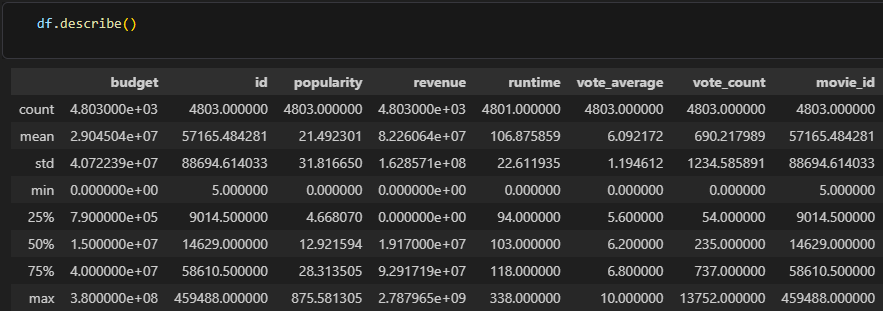
\includegraphics[width=0.9\linewidth]{immagini/describe}
\end{figure}
Per farlo, calcoliamo innanzitutto la somma dei valori "null" e dei valori presenti per ciascuna colonna, filtrando i risultati in modo da visualizzare solo quelli rilevanti. Ne approfittiamo anche per verificare la presenza di eventuali righe duplicate nel dataset. Infine, per avere un quadro visivo immediato, calcoliamo la percentuale di valori mancanti rispetto al totale e la rappresentiamo tramite un grafico a barre dedicato.
\begin{lstlisting}
	# Analisi dei valori mancanti e duplicati
	null_val = df.isnull().sum().sort_values(ascending=False)
	print("Valori Mancanti:")
	print(null_val[null_val > 0])
	
	present_val = df.notnull().sum().sort_values(ascending=False)
	print("\nValori Presenti:", present_val[present_val > 0])
	df_plot = pd.DataFrame({
		'Presenti': present_val,
		'Mancanti': null_val
	})
	
	print("\nDuplicati:", df.duplicated().sum())
	
	null_perc = (df.isnull().sum() / len(df)) * 100
	null_perc[null_perc > 0].plot(kind="bar", figsize=(15, 6), title="Percentuale dei Valori Mancanti")
	plt.ylim(0, 100)
	plt.xticks(rotation=45, ha="right")
	plt.show()
\end{lstlisting}
\begin{figure}[H]
	\centering
	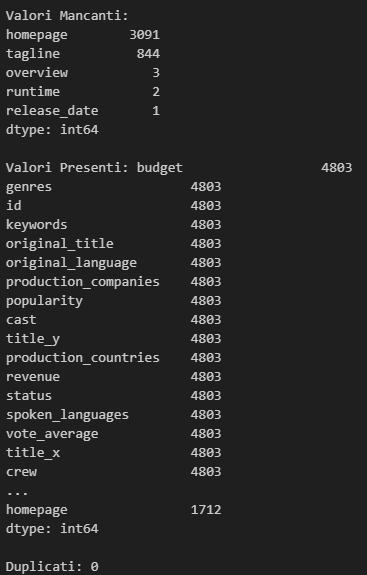
\includegraphics[width=0.3\linewidth]{immagini/null}
\end{figure}
\begin{figure}[H]
	\centering
	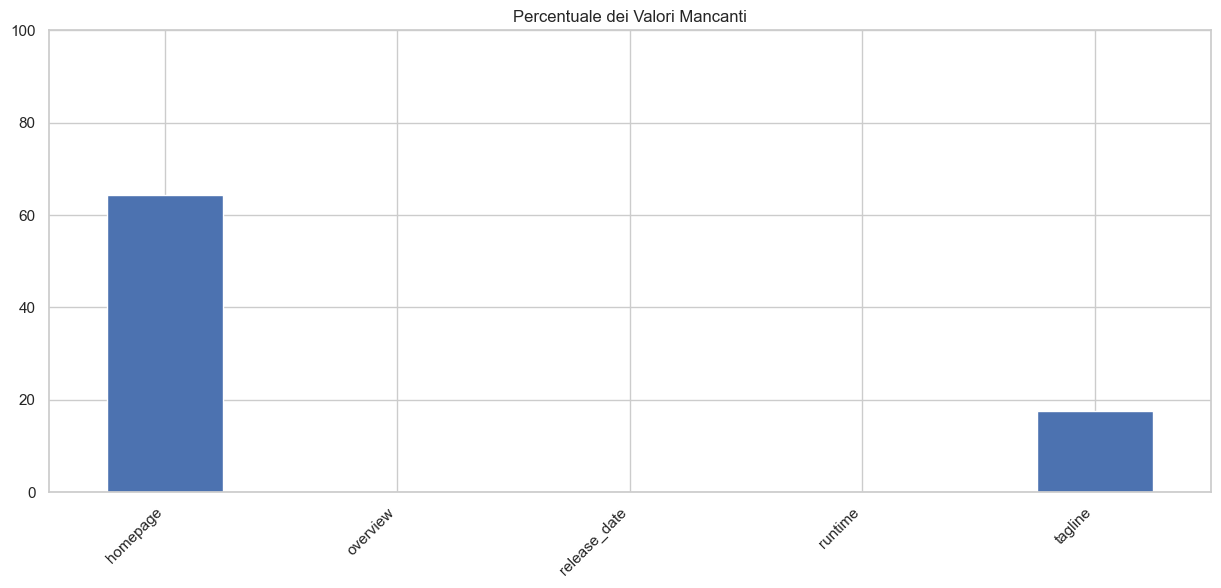
\includegraphics[width=0.9\linewidth]{immagini/nullgraph}
\end{figure}
Molte colonne del dataset si presentava originariamente sotto forma di stringhe di testo contenenti liste di dizionari, strutturate in modo simile a un formato JSON. Per rendere queste informazioni facilmente analizzabili, si \`e reso necessario estrarre solo il dato rilevante, ovvero il nome del genere, dell'attore o della casa di produzione, scartando i codici identificativi e altri metadati non necessari. A tale scopo, \`e stata definita la funzione personalizzata clean\_json. Questa funzione effettua innanzitutto un controllo preliminare per verificare che la cella contenga effettivamente del testo e non sia vuota, al fine di evitare anomalie e interruzioni nell'esecuzione del codice. Successivamente, attraverso l'utilizzo di un blocco di gestione degli errori utile a prevenire blocchi causati da eventuali stringhe corrotte, la funzione sfrutta il metodo literal\_eval della libreria ast per convertire in modo sicuro la stringa testuale in una reale struttura dati Python. A questo punto, tramite l'utilizzo di una list comprehension, viene effettuata un'iterazione sui dizionari per estrarre esclusivamente il testo associato alla chiave "name". Una volta definita la logica di estrazione, i nomi di tutte le colonne interessate sono stati raccolti all'interno di una lista dedicata. Infine, attraverso un ciclo iterativo e avvalendosi del metodo .apply(), la trasformazione \`e stata applicata in modo massivo a tutte le variabili selezionate, sovrascrivendo i dati grezzi originali con le nuove liste pulite direttamente all'interno del dataframe.
\begin{lstlisting}
	# Passaggio da json a lista di stringhe per le colonne specificate
	def clean_json(json_text):
	if pd.isna(json_text) or not isinstance(json_text, str):
	return []
	
	try:
	
	converted_list = ast.literal_eval(json_text)
	return [item["name"] for item in converted_list if "name" in item]
	except (ValueError, SyntaxError):
	return []
	
	colonne_json = [
	"genres",
	"keywords",
	"production_companies",
	"production_countries",
	"spoken_languages",
	"cast",
	"crew"
	]
	for col in colonne_json:
	df[col] = df[col].apply(clean_json)
	df.head() 
\end{lstlisting}

\subsection{Pulizia del Dataset}
Al fine di preparare il dataset per le successive esplorazioni, \`e stata eseguita una fase di pulizia e trasformazione dei dati. Inizialmente, la variabile relativa alla data di uscita \`e stata convertita in un formato temporale adeguato, gestendo in modo sicuro eventuali errori di formattazione e permettendo l'estrazione dell'anno di pubblicazione all'interno di una nuova colonna dedicata. Successivamente, per snellire la struttura delle informazioni, sono state rimosse alcune variabili ritenute non necessarie per lo scopo dell'analisi, come gli identificativi ridondanti, gli slogan promozionali, lo stato della produzione e i collegamenti alle pagine web. Si \`e poi proceduto all'eliminazione dei record privi del dato sulla durata della pellicola e alla normalizzazione del nome della colonna del titolo, correggendo le alterazioni dovute alla precedente unione dei dati. Per garantire la significativit\`a e l'affidabilità delle valutazioni finanziarie e qualitative, il dataframe \`e stato rigorosamente filtrato, conservando esclusivamente i film caratterizzati da budget, incassi e votazioni medie strettamente maggiori di zero. Infine, sfruttando i dati economici appena purificati, \`e stata generata una nuova metrica utile a calcolare il ritorno sull'investimento (ROI) in formato percentuale, indicatore fondamentale per misurare in modo standardizzato la profittabilit\`a economica di ciascuna opera cinematografica.
\begin{lstlisting}
	# Pulizia e trasformazione dei dati
	df["release_date"] = pd.to_datetime(df["release_date"], errors="coerce")
	df["year"] = df["release_date"].dt.year.astype("Int64")
	df = df.drop(["title_y", "tagline", "homepage", "movie_id", "status"], axis = 1)
	df = df.dropna(subset=["runtime"])
	df = df.rename(columns={"title_x": "title"})
	df = df[(df["budget"] > 0) & (df["revenue"] > 0) & (df["vote_average"] > 0)]
	df["roi"] = (df["revenue"] - df["budget"]) / df["budget"] * 100
\end{lstlisting}

\subsection{Visualizzazioni Grafiche}
Per approfondire la comprensione delle variabili a seguito della pulizia sono stati realizzati una serie di grafici a istogramma. Tali visualizzazioni consentono di esaminare la distribuzione, la dispersione e la frequenza dei dati relativi al budget, alla revenue, al runtime e ai ratings. 
\begin{itemize}
	\item Budget: Forte asimmetria positiva, il 75\% dei film ha un budget inferiore ai 40 milioni di dollari. Sulla destra si estende una coda sottile e allungata che rappresenta i rari blockbuster milionari;
	\item Revenue: Forte asimmetria positiva, pi\`u estrema rispetto al grafico precedente. Il 75\% dei film incassa meno di 93 milioni, ma presenta una coda molto lunga grazie al film Avatar, campione di incassi con 2,8 miliardi di dollari;
	\item Runtime: Classica distribuzione simile a una normale, con un picco centrale tra i 90 e 120 minuti, prevedibile da una media di 107. Ai lati di questo picco centrale le barre scendono mostrando pochissimi cortometraggi o film estesi;
	\item Vote Average: Distribuzione normale leggermente spostata a destra con voti molto bassi e che mostra la presenza di alcuni film ancora non valutati;
\end{itemize}
\begin{figure} [H]
	\centering
	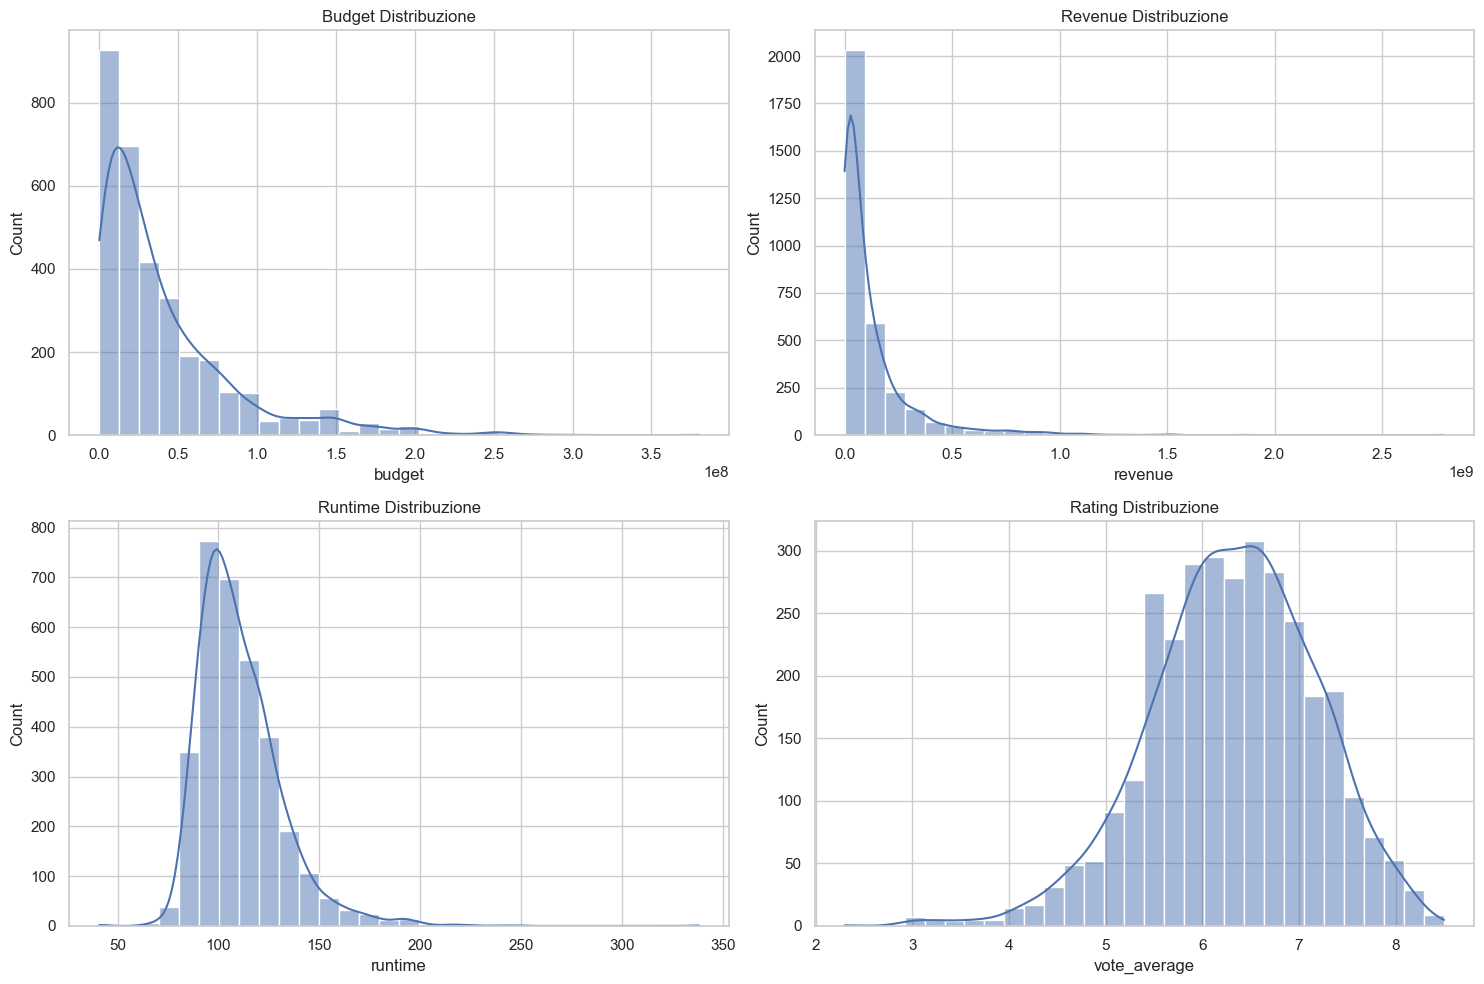
\includegraphics[width=1.0\linewidth]{immagini/histogram}
\end{figure}
Successivamente all'analisi delle distribuzioni, l'esplorazione visiva \`e proseguita con l'utilizzo di boxplot per le principali variabili numeriche. Questa tipologia di grafico offre una sintesi visiva estremamente efficace per valutare la dispersione dei dati, mettendo in evidenza la mediana, la variabilità e l'intervallo in cui si concentra la maggior parte dei valori. L'obiettivo principale di questa rappresentazione \`e l'identificazione degli outlier, ovvero quei valori anomali che si discostano in modo significativo dal corpo principale della distribuzione. Nel contesto cinematografico, l'osservazione dei boxplot permette di individuare e isolare facilmente le eccezioni statistiche, come i grandi blockbuster caratterizzati da investimenti o incassi straordinariamente elevati rispetto alla media del settore, oppure pellicole con durate e valutazioni estreme. Riconoscere e mappare queste anomalie statistiche risulta fondamentale per comprendere la reale eterogeneit\`a del dataset e per valutare in che misura tali eccezioni possano influenzare i modelli e le elaborazioni successive.
\begin{figure}[H]
	\centering
	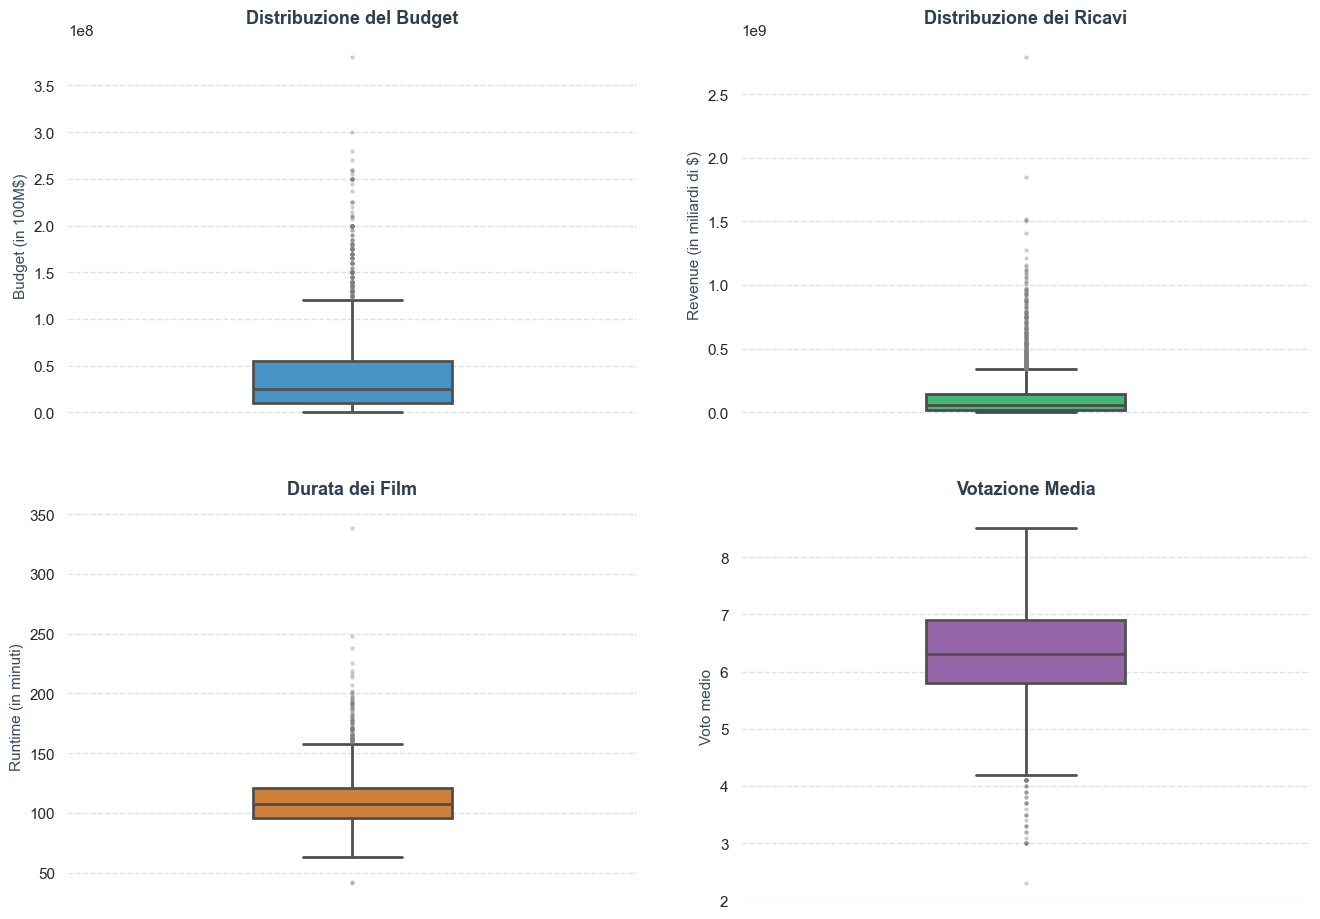
\includegraphics[width=0.9\linewidth]{immagini/boxplot}
\end{figure}
Attraverso la creazione di un grafico a barre, \`e stata possibile l'osservazione della tendenza storica, la quale mette in luce una presenza piuttosto marginale di pellicole risalenti ai primi decenni del Novecento, seguita da una crescita lenta e graduale che prende il via intorno agli anni Ottanta. Il dato visivo pi\`u rilevante emerge tuttavia a partire dalla fine degli anni Novanta, momento in cui si registra un'impennata quasi esponenziale della produzione cinematografica registrata, fino a raggiungere il picco massimo intorno alla metà degli anni 2010.
\begin{figure}[H]
	\centering
	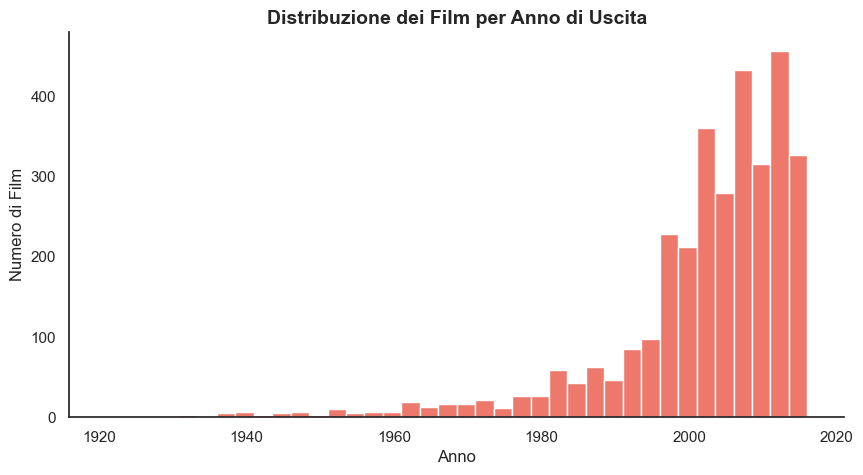
\includegraphics[width=0.8\linewidth]{immagini/uscite}
\end{figure}
Per arricchire l'analisi anche delle variabili di natura categoriale sono stati creati tre grafici a barre affiancati, isolando e quantificando la classifica delle prime 10 posizioni relative ai generi, ai membri del cast e alle case di produzione ordinati in base al numero complessivo di pellicole in cui compaiono.\\
Il primo grafico, dedicato ai generi cinematografici, evidenzia una netta predominanza dei film drammatici e delle commedie, seguiti a distanza dai thriller e dai film d'azione. Il secondo grafico sposta l'attenzione sulle presenze attoriali, mostrando in modo chiaro i volti pi\`u assidui all'interno del panorama analizzato, tra cui Samuel L. Jackson, Robert De Niro e Matt Damon con rispettivamente la presenza in 52, 47 e 45 film. L'ultimo grafico illustra invece il peso delle diverse case di produzione, confermando l'assoluto predominio e la forte presenza storica delle case di Hollywood quali Warner Bros, Universal Pictures e Paramount Pictures. 
\begin{figure}[H]
	\centering
	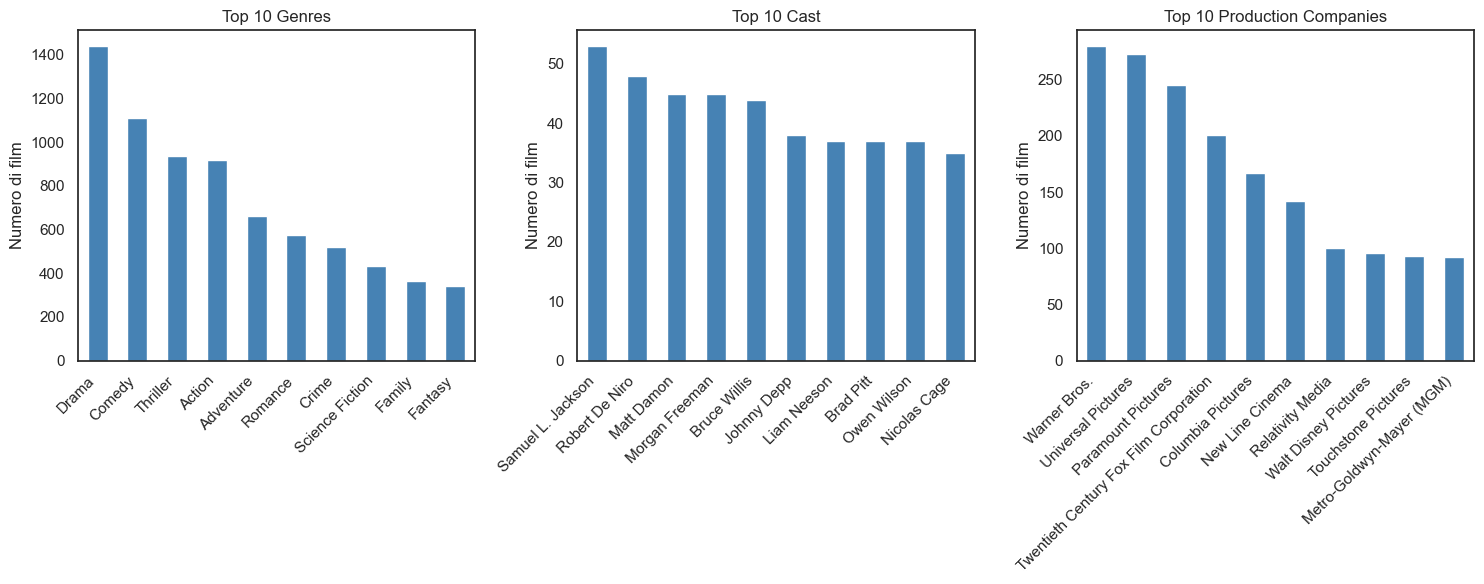
\includegraphics[width=1.0\linewidth]{immagini/top10}
\end{figure}
\begin{lstlisting}
	Generi totali: 19
	Top 10 generi:
	Drama              1439
	Comedy             1110
	Thriller            935
	Action              918
	Adventure           661
	Romance             574
	Crime               520
	Science Fiction     431
	Family              365
	Fantasy             342
\end{lstlisting}
Il seguente grafico si focalizza invece sul ritorno sull'investimento mediano in funzione del genere. Dall'osservazione di questa metrica emerge che le pellicole in grado di garantire in media i ritorni percentuali più elevati sono i documentari, seguiti a breve distanza dalle opere musicali e dai film horror. Questa spiccata efficienza economica è tipicamente riconducibile ai costi di produzione molto pi\`u contenuti che caratterizzano queste produzioni. Al contrario, generi che richiedono per natura budget più elevati per effetti visivi e campagne markenting, come fantascienza e fantasy, si posizionano alla fine di questa classifica.
\begin{figure}[H]
	\centering
	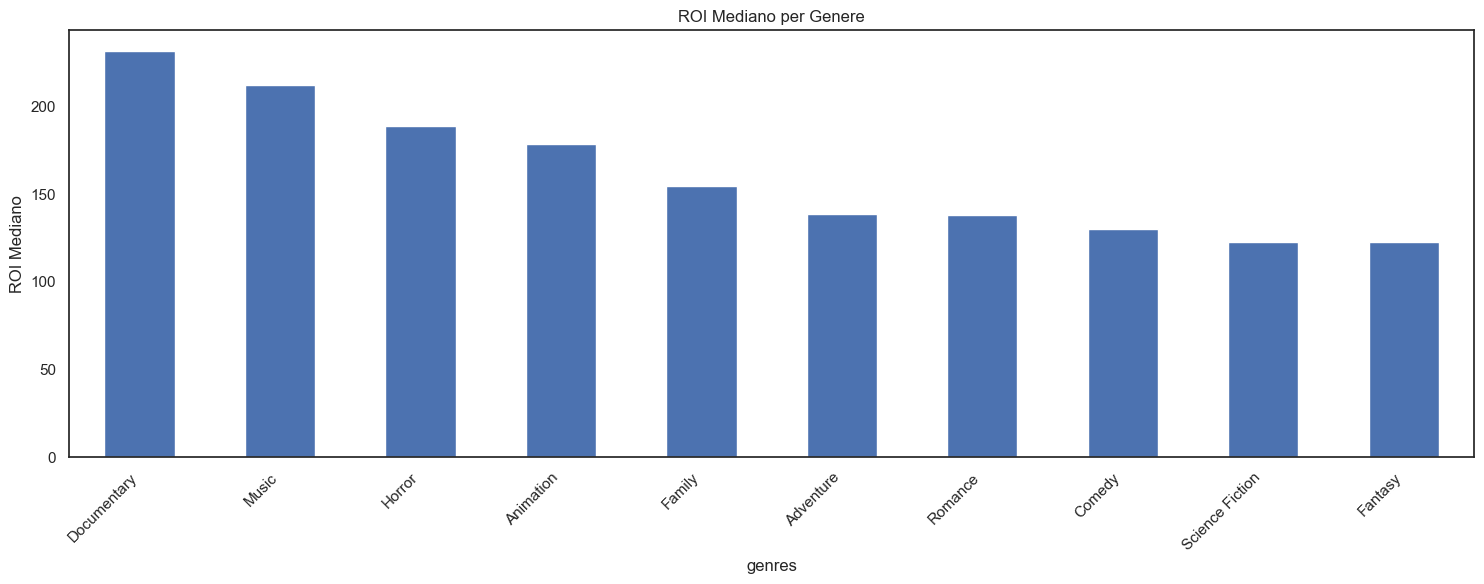
\includegraphics[width=1.0\linewidth]{immagini/roimed}
\end{figure}
Al fine di identificare i maggiori successi commerciali, \`e stato predisposto un grafico a barre che illustra i primi dieci film per volume di incassi globali. La visualizzazione evidenzia il netto primato isolato di Avatar, l'unica opera a sfiorare i 2,8 miliardi di dollari, seguita a debita distanza da Titanic. Il resto della graduatoria risulta invece fortemente dominato da noti franchise e blockbuster seriali che si attestano tutti stabilmente sopra la significativa soglia del miliardo di dollari di ricavi, delineando chiaramente i titoli a più alta redditività storica all'interno del campione.
\begin{figure}[H]
	\centering
	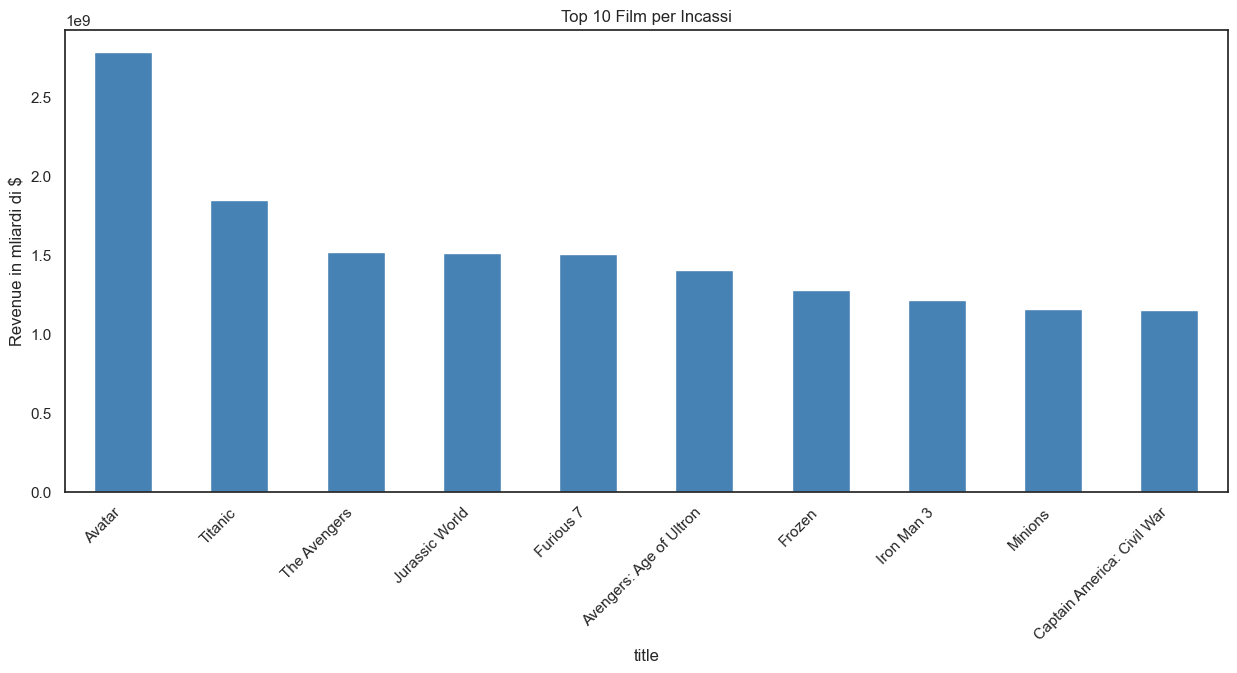
\includegraphics[width=1.0\linewidth]{immagini/topincassi}
\end{figure}

\subsection{Correlazioni}
Per approfondire le relazioni lineari tra le metriche quantitative del dataset, la matrice di correlazione offre una quantificazione precisa dei legami statistici attraverso i rispettivi coefficienti numerici. Emerge in modo evidente una forte associazione positiva, pari a 0.71, tra il budget stanziato e i ricavi generati, a dimostrazione del fatto che investimenti finanziari pi\`u cospicui tendono a tradursi in maggiori incassi al botteghino. Si rileva inoltre una significativa correlazione positiva tra gli incassi e l'indice di popolarit\`a (0.60), suggerendo che il successo commerciale sia strettamente connesso alla risonanza mediatica dell'opera. Al contrario, la variabile del ritorno sull'investimento presenta valori stabilmente prossimi allo zero con tutte le altre metriche, confermando analiticamente che la redditività percentuale prescinde dalla scala economica assoluta del progetto cinematografico.\\
Questo scenario trova un riscontro visivo diretto nel grafico a dispersione adiacente, in cui la distribuzione della nuvola di punti si sviluppa diagonalmente verso l'alto, convalidando la tendenza alla crescita dei ricavi in concomitanza con l'aumento dei costi di produzione. L'integrazione di una scala cromatica legata alla votazione media arricchisce la lettura del grafico con una dimensione qualitativa, evidenziando come le pellicole maggiormente apprezzate dal pubblico, contraddistinte dalle tonalit\`a più chiare e accese, tendano a concentrarsi prevalentemente nelle fasce di incasso medio-alte, pur non escludendo la presenza di produzioni a basso budget capaci di ottenere eccellenti valutazioni critiche.
\begin{figure}[H]
	\centering
	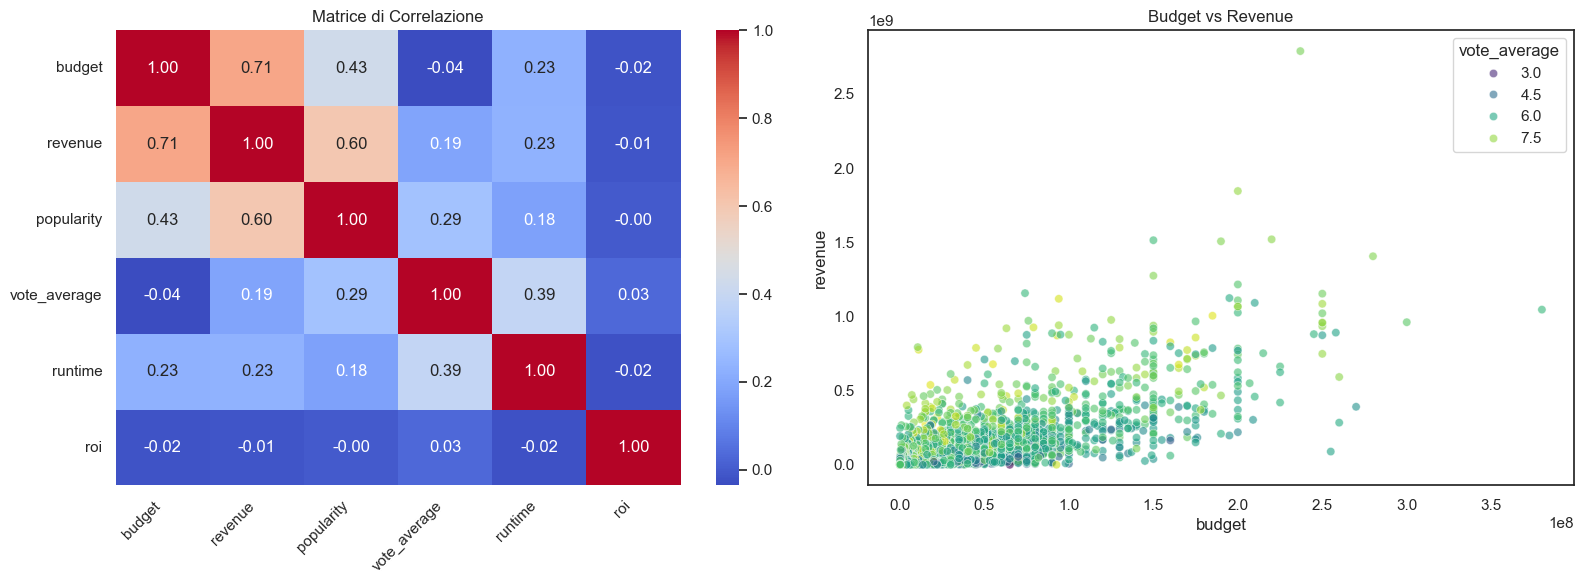
\includegraphics[width=1.0\linewidth]{immagini/corr}
\end{figure}

Per tracciare un quadro storico dell'evoluzione finanziaria del settore cinematografico, \`e stato sviluppato un grafico a linee che pone a confronto l'andamento del budget medio e dell'incasso medio nel corso dei decenni.\\
La curva dedicata al budget medio (in rosso) mostra una stabilit\`a quasi assoluta dal 1940 fino alla fine degli anni Settanta, mantenendosi su livelli storicamente molto contenuti. A partire dagli anni Ottanta, tuttavia, l'investimento medio intraprende una crescita costante e progressiva che accelera sensibilmente nel nuovo millennio, riflettendo chiaramente l'avvento dei moderni blockbuster e il generale aumento dei costi di produzione e di marketing.\\
Al contrario, la linea degli incassi medi (in verde) rivela una forte volatilit\`a nei primi quarant'anni della linea temporale. Questa spiccata oscillazione, caratterizzata da picchi isolati e bruschi cali, \`e legata con ogni probabilit\`a alla scarsità di dati per i film pi\`u datati, dove il successo straordinario di una singola pellicola era in grado di alterare drasticamente la media del rispettivo anno.\\
L'elemento analitico pi\`u rilevante si osserva a partire dagli anni Novanta: pur mantenendo una forte componente fluttuante, la curva dei ricavi sperimenta un'impennata notevole, distanziando in modo sistematico quella dei costi. Il progressivo ampliamento della forbice tra entrate e uscite nell'ultimo ventennio evidenzia la straordinaria capacit\`a del mercato cinematografico contemporaneo di massimizzare i profitti su scala globale, portando gli incassi medi verso il picco storico in prossimità della fine della linea temporale.
\begin{figure}[H]
	\centering
	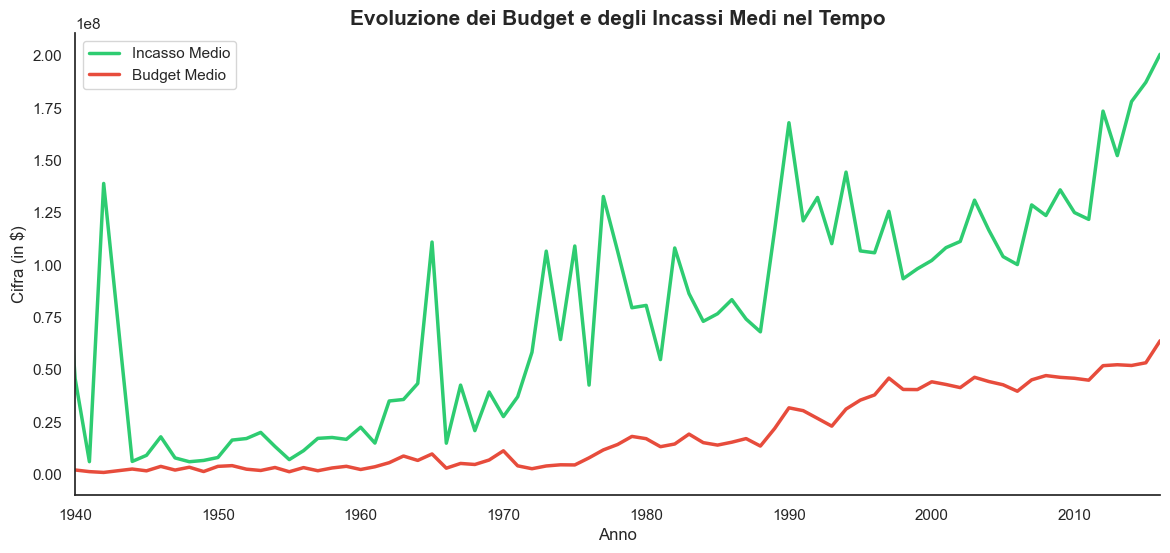
\includegraphics[width=1.0\linewidth]{immagini/corr2}
\end{figure}

\subsection{Wordcloud}
Per esplorare le tematiche ricorrenti e i nuclei narrativi che caratterizzano le produzioni cinematografiche del dataset, \`e stata realizzata una wordcloud focalizzata sui termini pi\`u frequenti all'interno delle trame dei film. L'analisi visiva mette immediatamente in luce i motori concettuali ed emotivi universali del cinema: parole di grandi dimensioni come "life", "find", "world" e "family" indicano chiaramente come la stragrande maggioranza delle sceneggiature si sviluppi attorno a percorsi di ricerca, dinamiche relazionali e contesti esistenziali o d'azione di ampio respiro.\\
Accanto a questi pilastri macrotematici, si nota una forte concentrazione di termini legati ai legami interpersonali e agli archetipi dei personaggi, quali "man", "young", "father", "friend" e "love" — che testimoniano la centralità dei conflitti familiari e delle evoluzioni sentimentali nelle storie. Infine, la ricorrenza di marcatori di contesto come "time", "new", "town" e "home" delinea la cornice spaziale e temporale tipica in cui prendono vita le vicende. Nel complesso, la visualizzazione restituisce una mappatura semantica coerente, confermando come l'industria cinematografica si affidi a tropi e concetti universali per garantire l'immediata immedesimazione e l'efficacia comunicativa sul pubblico globale.
\begin{figure}[H]
	\centering
	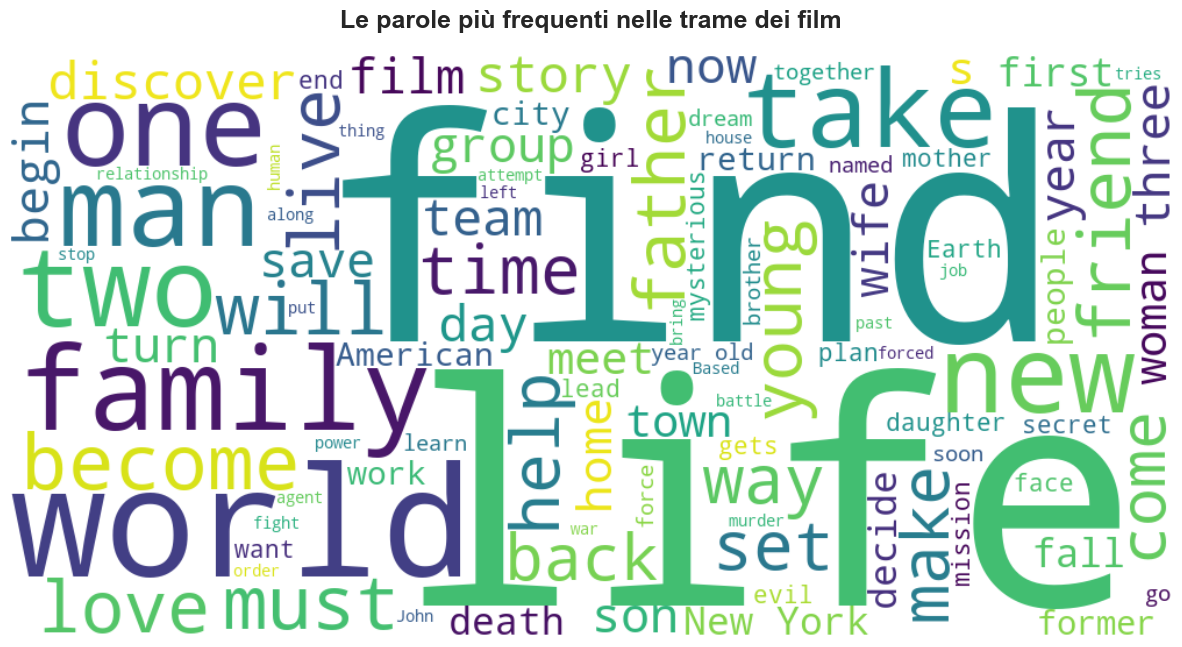
\includegraphics[width=0.8\linewidth]{immagini/cloud}
\end{figure}

\section{Svolgimento del Progetto}
\subsection{Preparazione del Dataset}
\subsubsection{Funzione: clean\_json}
L'avvio del progetto ha richiesto una cruciale fase preliminare di pulizia e pre-elaborazione dei dati, mirata a normalizzare la struttura delle variabili categoriali pi\`u complesse presenti nel dataset, come i generi cinematografici, i membri del cast e le case di produzione. Molte di queste informazioni, infatti, si presentavano originariamente sotto forma di stringhe testuali contenenti strutture dati nidificate e formattate in modo simile a frammenti JSON. Per poter manipolare e quantificare agevolmente queste informazioni, si \`e reso necessario sviluppare una specifica funzione di parsing denominata clean\_json. Sfruttando il modulo ast (Abstract Syntax Trees) per convertire in sicurezza la stringa in una struttura nativa Python, la funzione analizza la lista di dizionari cos\`i ottenuta ed estrae da ciascun elemento esclusivamente il valore associato alla chiave utile, in questo caso il nome dell'attributo. Questo processo di estrazione consente di trasformare blocchi di testo complessi in semplici liste di stringhe pulite, ponendo le basi strutturali fondamentali per tutte le successive analisi statistiche e visualizzazioni grafiche.
\begin{lstlisting}
	def clean_json(json_text):
		list_names = []
		converted_list = ast.literal_eval(json_text)
		for item in converted_list:
		list_names.append(item["name"])
		return list_names
\end{lstlisting}

\subsubsection{Funzione: cleaning\_and\_processing}
A valle della definizione della logica di estrazione testuale, il processo di preparazione dei dati si è concretizzato nella strutturazione di una pipeline complessiva di pulizia e pre-elaborazione, racchiusa all'interno della funzione cleaning\_and\_preprocessing. L'operazione iniziale di questa routine mira a garantire la solidità del dataset attraverso la rimozione automatica di tutti i record contenenti valori mancanti o nulli. Successivamente, l'attenzione si sposta sulla standardizzazione delle informazioni temporali: la colonna relativa alla data di uscita delle pellicole viene prima forzata in un formato data coerente (gestendo eventuali errori di conversione) e subito dopo riorganizzata visivamente secondo lo standard europeo basato su giorno, mese e anno.\\
Dopo aver risolto alcune ridondanze di nomenclatura, come la rinomina della colonna del titolo per una maggiore chiarezza formale, il cuore della funzione entra in gioco applicando massivamente la precedente routine clean\_json a tutte le variabili complesse. Questo passaggio permette di estrarre e appiattire in modo automatico le informazioni contenute in colonne fondamentali quali i generi, il cast, la troupe, le parole chiave, le case di produzione e le lingue parlate. Nel caso specifico dei generi cinematografici, viene integrata un'ulteriore accortezza per l'omogeneità dei dati, convertendo ogni termine estratto in minuscolo per prevenire discrepanze durante le future fasi di raggruppamento. Infine, la pipeline di lavoro si conclude con una fase di snellimento strutturale: tramite l'eliminazione mirata di quelle colonne ritenute ridondanti o non in linea con i successivi obiettivi di analisi (come gli identificativi numerici, i titoli duplicati e alcune variabili geografiche o finanziarie non necessarie in questo step), la funzione restituisce un dataframe perfettamente pulito, compatto e pronto per essere esplorato statisticamente.
\begin{lstlisting}
	def cleaning_and_preprocessing(df):
		df.dropna(inplace=True)
		df["release_date"] = pd.to_datetime(df["release_date"], errors='coerce')
		df["release_date"] = df["release_date"].dt.strftime('%d/%m/%Y')
		df.rename(columns={"title_x": "title"}, inplace=True)
		df["genres"] = df["genres"].apply(clean_json)
		df["genres"] = df["genres"].apply(lambda x: [genere.lower() for genere in x])
		df["keywords"] = df["keywords"].apply(clean_json)
		df["cast"] = df["cast"].apply(clean_json)
		df["crew"] = df["crew"].apply(clean_json)
		df["production_companies"] = df["production_companies"].apply(clean_json)
		df["production_countries"] = df["production_countries"].apply(clean_json)
		df["spoken_languages"] = df["spoken_languages"].apply(clean_json)
		df.drop(["id", "movie_id", "title_y", "budget", "revenue", "production_countries"], axis=1, inplace=True)
		return df
\end{lstlisting}

\subsubsection{Funzione: join\_list\_elements}
Come ultimo passaggio della fase di preparazione e formattazione dei dati, si \`e resa necessaria un'operazione di consolidamento delle variabili precedentemente estratte. A tale scopo è stata implementata la funzione join\_list\_elements, concepita per trasformare le strutture a lista in formati testuali lineari e immediatamente leggibili. La routine accetta in ingresso il dataframe e un elenco specifico di colonne su cui operare, iterando su ciascuna di esse in modo sistematico. Attraverso l'applicazione di una funzione lambda, il codice verifica dinamicamente la natura di ogni singolo elemento: qualora si tratti di una lista (come nel caso dei molteplici generi, degli attori o delle parole chiave associati a una singola pellicola), i suoi componenti vengono concatenati in un'unica stringa continua, separati da una virgola e da uno spazio; in caso contrario, il dato viene convertito in modo precauzionale in un formato testuale standard. Questa trasformazione finale risulta strategica non solo per migliorare la leggibilità diretta e l'esplorazione visiva del dataset, ma anche per predisporre le variabili categoriali a eventuali esportazioni in formato tabellare o a successive elaborazioni algoritmiche basate sull'analisi del testo, garantendo la massima compatibilità e coerenza strutturale.
\begin{lstlisting}
	def join_list_elements(dataframe, columns):
		for col in columns:
		dataframe[col] = dataframe[col].apply(
		lambda x: ", ".join(x) if isinstance(x, list) else str(x)
		)
		return dataframe
\end{lstlisting}
\subsubsection{Caricamento e Pulizia}
A completamento della fase di preparazione, il blocco principale del codice orchestra l'integrazione iniziale e il salvataggio dei dati. I due dataset nativi relativi a pellicole e crediti vengono caricati e fusi in un unico dataframe coerente attraverso il raccordo dei rispettivi identificativi numerici. Su questa struttura unificata viene poi applicata la pipeline di pulizia descritta in precedenza; infine, il dataset normalizzato viene esportato in un nuovo file CSV, garantendo la persistenza di un archivio pulito e già pronto per le successive fasi di analisi statistica.
\begin{lstlisting}
	movies = pd.read_csv("Dataset/tmdb_5000_movies.csv")
	credits = pd.read_csv("Dataset/tmdb_5000_credits.csv")
	df = pd.merge(movies, credits, left_on="id", right_on="movie_id")
	
	df = cleaning_and_preprocessing(df)
	df.to_csv('tmdb_5000_pulito.csv', index=False)
	print("Dataset salvato con successo!")
\end{lstlisting}

\subsection{Sentence Embedding}
Questa sezione del progetto avvia la fase di modellazione e arricchimento delle caratteristiche (feature engineering), finalizzata a trasformare il patrimonio informativo testuale in elementi computabili dall'algoritmo. Inizialmente, la funzione join\_list\_elements viene applicata per consolidare in stringhe lineari i metadati relativi a parole chiave, cast, troupe e case cinematografiche. Parallelamente, lo script estrae e ordina i generi univoci del dataset e genera una colonna accessoria contenente l'acronimo in minuscolo di ciascun titolo, utile per supportare logiche di ricerca rapida.\\
Il passaggio chiave per l'analisi semantica consiste nella creazione di una variabile testo omnicomprensiva, denominata sentence\_var. Questa stringa unisce tutti i descrittori di un film: titolo, trama (overview), parole chiave, slogan (tagline), generi, attori, membri chiave della troupe e produttori. Questo blocco unico di testo viene infine dato in pasto al modello SentenceTransformer che, tramite il metodo encode, ne esegue la vettorializzazione, restituendo una matrice di embedding pronti per il calcolo della similarità.\\
Nel campo dell'elaborazione del linguaggio naturale, il sentence embedding rappresenta il processo di mappatura di stringhe di testo di lunghezza variabile (frasi, paragrafi o interi documenti) in vettori numerici densi a dimensione fissa.\\
A differenza dei modelli classici come la Bag-of-Words o TF-IDF che si limitano a contare la presenza delle parole creando matrici sparse e prive di senso logico, i sentence embedding sono progettati per catturare il contesto e il significato semantico. L'obiettivo fondamentale \`e fare in modo che la distanza geometrica tra due vettori nello spazio multidimensionale rifletta la somiglianza concettuale dei testi di partenza. Di conseguenza, due film che descrivono trame simili utilizzando sinonimi o vocaboli completamente diversi saranno comunque mappati in punti molto vicini dello spazio vettoriale, consentendo di superare i limiti della rigida ricerca per parole chiave.
\begin{lstlisting}
	df = join_list_elements(df, ["keywords", "cast", "crew", "production_companies"])
	
	all_genres = [genres for sublist in df["genres"] for genres in sublist]
	unique_genres = sorted(list(set(all_genres)))
	#print(f"Generi individuati:{unique_genres}")
	
	df["acronym"] = df["title"].str.lower().str.split().apply(
	lambda parole: "".join([parola[0] for parola in parole]) if isinstance(parole, list) else ""
	)
	#print(df[["title", "acronym"]].head())
	
	genres_str = df["genres"].apply(lambda x: " ".join(x) if isinstance(x, list) else "")
	
	sentence_var = (df["title"] + " " + df["overview"] + " " + df["keywords"] + " " + df["tagline"] + " " + genres_str + " " + df["cast"] + " " + df["crew"] + " " + df["production_companies"]) 
	model = SentenceTransformer('all-MiniLM-L6-v2')
	embeddings_sentence = model.encode(sentence_var.tolist(), convert_to_numpy=True)
\end{lstlisting}
\subsection{Calcolo delle Metriche}
\subsubsection{Funzione: calc\_sentence\_score}
Per tradurre l'input testuale dell'utente in un valore metrico direttamente computabile, \`e stata implementata la funzione calc\_sentence\_score. Questa routine riceve la query espressa in linguaggio naturale e, come prima operazione, la converte in un vettore denso sfruttando il medesimo modello di Sentence Transformer utilizzato per l'indicizzazione del catalogo cinematografico, garantendo così la coerenza dello spazio vettoriale. Successivamente, viene calcolata la cosine similarity tra l'embedding della richiesta e la matrice precomputata di tutte le pellicole, determinando la vicinanza geometrica e quindi l'affinit\`a concettuale tra i testi. Poich\`e questo coefficiente statistico oscilla originariamente all'interno di un intervallo compreso tra -1 e 1, il codice introduce un passaggio cruciale di normalizzazione attraverso la tecnica del Min-Max scaling. Riscalmando matematicamente i vettori in modo che la minor somiglianza rilevata corrisponda a 0 e la maggiore a 1, la funzione restituisce un vettore di punteggi standardizzato e perfettamente calibrato. 
\begin{lstlisting}
	def calc_sentence_score(user_query):
		query_embedding = model.encode([user_query], convert_to_numpy=True)
		sentence_cosine = cosine_similarity(query_embedding, embeddings_sentence)[0]
	
		sentence_score_normalized = (sentence_cosine - sentence_cosine.min()) / (sentence_cosine.max()-sentence_cosine.min())
		return sentence_score_normalized
\end{lstlisting}

\subsubsection{Funzione: find\_genres}
Al fine di intercettare in modo mirato le preferenze categoriali espresse esplicitamente dall'utente, è stata sviluppata la funzione find\_genres. Questa routine esegue una scansione della richiesta testuale per verificare la presenza diretta di specifici generi cinematografici all'interno del linguaggio naturale. Come prima operazione, l'input viene interamente normalizzato in caratteri minuscoli per garantire la totale insensibilit\`a alle maiuscole ed evitare mancate corrispondenze. Successivamente, la funzione confronta la stringa cos\`i elaborata con l'elenco dei generi univoci precedentemente mappati nel dataset, estraendo ogni termine che compaia come sottostringa all'interno della richiesta. Questo meccanismo di filtraggio basato su parole chiave esplicite risulta di fondamentale importanza strategica per il motore di ricerca, in quanto permette di isolare i desiderata categorici dell'utente prima delle successive fasi algoritmiche. In questo modo, il sistema ottiene un elenco pulito di generi di riferimento che pu\`o essere utilizzato per applicare filtri booleani rigidi o logiche di potenziamento dei punteggi, affiancando alla comprensione puramente semantica degli embedding un controllo tassonomico preciso e deterministico.
\begin{lstlisting}
	def find_genres(user_query, unique_genres):
		query_lowered = user_query.lower()
		genres_found = [gen for gen in unique_genres if gen in query_lowered]
		return genres_found
\end{lstlisting}

\subsubsection{Funzione: calc\_genres\_score}
Per valorizzare la congruenza tassonomica tra le richieste espresse dall'utente e il catalogo a disposizione, \`e stata implementata la funzione calc\_genres\_score. Questa routine ha il compito di quantificare l'affinità categoriale assegnando un punteggio matematico basato sulla sovrapposizione dei generi cinematografici. Il codice cicla attraverso tutte le pellicole del dataframe e valuta lo scenario di partenza: qualora l'elenco dei generi estratti dalla query risulti vuoto, viene assegnato di default un punteggio pari a zero a ogni riga, neutralizzando l'impatto di questa metrica. Nel caso in cui l'utente abbia invece specificato uno o pi\`u generi di interesse, la funzione calcola l'intersezione logica tra l'insieme dei desiderata e l'insieme dei generi associati al singolo film. Questo valore viene successivamente normalizzato dividendolo per il numero totale di generi richiesti dall'utente, generando cos\`i un indice standardizzato compreso tra 0 e 1 che rappresenta la percentuale esatta di soddisfacimento dei requisiti. Questo punteggio deterministico agisce come un moltiplicatore di rilevanza all'interno del motore complessivo, permettendo al sistema di premiare e spingere verso l'alto i titoli che rispettano in modo rigoroso i vincoli categorici indicati esplicitamente nella query.
\begin{lstlisting}
	def calc_genres_score(query_genres):
		genres_score = []
		for genres in df["genres"]:
			if len(query_genres) == 0:
				genres_score.append(0)
			else:
				intersection = set(query_genres) & set(genres)
				num_genres = len(intersection) / len (query_genres)
				genres_score.append(num_genres)
		return genres_score
\end{lstlisting}

\subsubsection{Funzione: calc\_title\_score}
Per integrare la ricerca diretta dei titoli all'interno della logica di raccomandazione, la funzione calc\_title\_score implementa una strategia di corrispondenza multi-livello che valuta l'affinit\`a tra la richiesta dell'utente e il catalogo. Dopo aver normalizzato la query in caratteri minuscoli, l'algoritmo calcola in parallelo tre indici di somiglianza, estraendo per ciascun film il valore massimo ottenuto: una corrispondenza esatta, una concordanza deterministica con gli acronimi e un punteggio testuale di tipo fuzzy. Quest'ultimo approccio si fonda sulla Distanza di Levenshtein, una metrica matematica che quantifica il numero minimo di modifiche (inserimenti, cancellazioni o sostituzioni) necessarie per trasformare una stringa in un'altra. Superando la rigidit\`a della logica booleana dicotomica, la ricerca fuzzy valuta il grado di somiglianza, tollerando variazioni o lievi errori di battitura. Nello specifico, l'utilizzo della variante partial\_ratio ottimizza il confronto tra testi di lunghezze differenti, verificando se la query, tipicamente pi\`u corta, corrisponde in modo ottimale a una specifica porzione del titolo del film. L'unione di queste tre metriche garantisce un motore di riconoscimento robusto e flessibile, capace di individuare l'opera desiderata anche a fronte di imprecisioni o acronimi.
\begin{lstlisting}
	def calc_title_score(user_query, df):
		query_normalized = user_query.lower()
		titoli_lower = df["title"].str.lower()
		
		exact_match = titoli_lower.str.contains(query_normalized, regex=False).astype(float)
		
		acronym_match = (df["acronym"] == query_normalized).astype(float)
		
		fuzzy_match = titoli_lower.apply(lambda x: fuzz.partial_ratio(query_normalized, x) / 100.0)
		
		best_title_score = np.maximum.reduce([exact_match, acronym_match, fuzzy_match])
		return best_title_score
\end{lstlisting}

\subsubsection{Funzione: calc\_people\_score}
Per intercettare i riferimenti a specifiche figure umane o societarie menzionate dall'utente, la funzione calc\_people\_score estende la logica di confronto testuale ai metadati relativi al cast, alla troupe cinematografica e alle case di produzione. Il codice unifica inizialmente queste tre informazioni in un unico blocco di testo normalizzato in caratteri minuscoli, azzerando l'influenza delle maiuscole. Su questa stringa combinata vengono calcolati in parallelo due distinti indici di somiglianza rispetto alla query: una verifica di corrispondenza esatta, che rileva la presenza diretta del nome cercato e un confronto di tipo fuzzy basato sempre sulla metrica del partial\_ratio. Quest'ultimo strumento si rivela essenziale per identificare correttamente registi, attori o marchi editoriali anche in presenza di refusi, omissioni o grafie parziali di nomi complessi. Attraverso l'applicazione della funzione np.maximum, il sistema seleziona infine il valore più elevato tra i due punteggi ottenuti per ciascuna pellicola, garantendo una valutazione ottimale dell'affinit\`a e fornendo al motore di raccomandazione una metrica robusta per premiare i titoli legati ai professionisti del cinema desiderati dall'utente.
\begin{lstlisting}
	def calc_people_score(user_query, df):
		query_normalized = user_query.lower()
		people_lower = (df["cast"] + " " + df["crew"]+ " " + df["production_companies"]).str.lower()
		query_normalized_lower = query_normalized.lower()
		exact_match = people_lower.str.contains(query_normalized_lower, regex=False).astype(float)
		fuzzy_match = people_lower.apply(lambda x: fuzz.partial_ratio(query_normalized_lower, x) / 100.0)
		people_score = np.maximum(exact_match, fuzzy_match)
		return people_score
\end{lstlisting}

\subsubsection{Funzione: calc\_total\_score}

\begin{lstlisting}
	def calc_total_score(sentence_score_normalized, genres_score, best_title_score, best_people_score):
		sentence_arr = np.array(sentence_score_normalized)
		genres_arr = np.array(genres_score)
		title_arr = np.array(best_title_score)
		people_arr = np.array(best_people_score)
		
		w_title = 0.3
		w_people = 0.2
		w_genres = 0.2
		w_sentence = 0.3
		
		if best_title_score.max() < 0.7:
		w_people += 0.20
		w_genres += 0.10
		w_title = 0.0
		
		if best_people_score.max() < 0.7:
		w_sentence += w_people
		w_people = 0.0
		# Se è il cast o la produzione
		if best_people_score.max() >= 0.7:
		w_sentence = 0.2
		w_people = 0.3
		
		total_score = (
		(sentence_arr * w_sentence) +
		(genres_arr * w_genres) +
		(title_arr * w_title) +
		(people_arr * w_people)
		)
		
		return total_score
\end{lstlisting}

\subsubsection{Ricerca dei Film}

\begin{lstlisting}
	def search_film():
		user_query = input("Inserisci la tua query: ")
		
		sentence_score = calc_sentence_score(user_query)
		
		query_genres = find_genres(user_query, unique_genres)
		genres_score = calc_genres_score(query_genres)
		
		best_title_score = calc_title_score(user_query, df)
		
		best_people_score = calc_people_score(user_query, df)
		
		total_score = calc_total_score(sentence_score, genres_score, best_title_score, best_people_score)
		results = list(enumerate(total_score))
		top_10 = sorted(results, key=lambda x: x[1], reverse=True)[:10]
		index = [i[0] for i in top_10]
		table = df.iloc[index][["title", "genres", "cast", "production_companies"]]
		print("\nFilm Consigliati per te in base alla tua query: {}".format(user_query))
		return table
\end{lstlisting}
\begin{figure}[H]
	\centering
	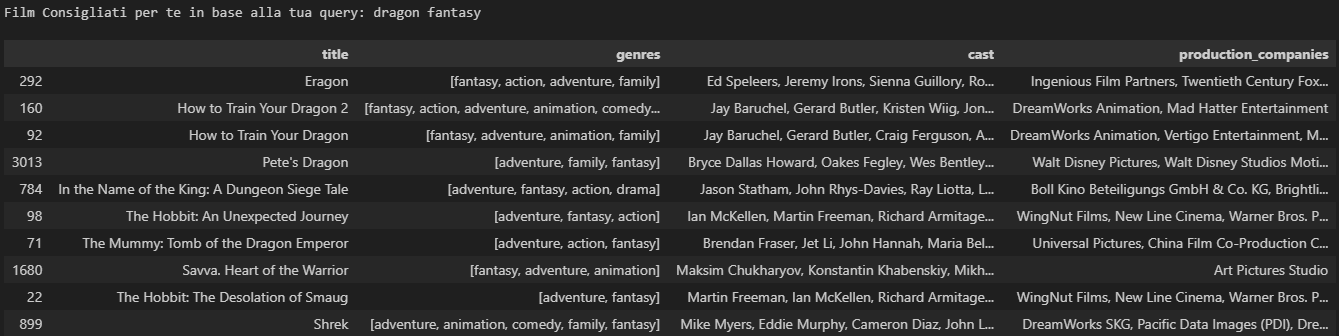
\includegraphics[width=1\linewidth]{immagini/search}
\end{figure}

\section{Validazione}
\subsection{Funzione: get\_top\_k\_titles}
\begin{lstlisting}
	def get_top_k_titles(user_query, k=10):
		query_genres = find_genres(user_query, unique_genres)
		genres_score = calc_genres_score(query_genres)
		
		query_pure = user_query.lower()
		for gen in query_genres:
		query_pure = query_pure.replace(gen, "").strip()
		if not query_pure: query_pure = user_query.lower()
		
		sentence_score = calc_sentence_score(user_query)
		best_title_score = calc_title_score(query_pure, df)
		best_people_score = calc_people_score(query_pure, df)
		
		total_score = calc_total_score(sentence_score, genres_score, best_title_score, best_people_score)
		results = list(enumerate(total_score))
		top_k = sorted(results, key=lambda x: x[1], reverse=True)[:k]
		
		return [df.iloc[i[0]]["title"] for i in top_k]
\end{lstlisting}

\subsection{Validation Set}

\begin{lstlisting}
	validation_set = [
	# Query basilari
	{
		"query": "action robert downey jr.", 
		"expected": ["Iron Man", "The Avengers"]
	},
	{
		"query": "animation jesse eisenberg", 
		"expected": ["Rio", "Rio 2"]
	},
	{
		"query": "christopher nolan space", 
		"expected": ["Interstellar"]
	},
	{
		"query": "pirates johnny dep", 
		"expected": ["Pirates of the Caribbean: The Curse of the Black Pearl"]
	},
	{
		"query": "trein your dregon",
		"expected": ["How to Train Your Dragon"]
	},
	{
		"query": "zoe saldana action",
		"expected": ["Guardians of the Galaxy", "Avatar"]
	},
	
	# Query miste con generi e attori
	{
		"query": "romance leonardo dicaprio", 
		"expected": ["Titanic", "The Great Gatsby"]
	},
	{
		"query": "sci-fi keanu reeves", 
		"expected": ["The Matrix", "The Matrix Reloaded"]
	},
	{
		"query": "action tom cruise", 
		"expected": ["Mission: Impossible", "Mission: Impossible II", "Mission: Impossible III", "Edge of Tomorrow"]
	},
	{
		"query": "kristen bell animation", 
		"expected": ["Frozen"]
	},
	{
		"query": "action adventure fantasy sam worthington", 
		"expected": ["Avatar", "Clash of the Titans"]
	},
	
	# Query con registi e trame
	{
		"query": "christopher nolan dream", 
		"expected": ["Inception"]
	},
	{
		"query": "quentin tarantino crime story", 
		"expected": ["Pulp Fiction", "Reservoir Dogs"]
	},
	{
		"query": "steven spielberg dinosaur park", 
		"expected": ["Jurassic Park"]
	},
	{
		"query": "peter jackson ring fantasy", 
		"expected": ["The Lord of the Rings: The Fellowship of the Ring", "The Lord of the Rings: The Two Towers", "The Lord of the Rings: The Return of the King"]
	},
	
	# Query con brand e case di produzione
	{
		"query": "pixar animation", 
		"expected": ["Cars", "A Bug's Life"]
	},
	{
		"query": "marvel studios action", 
		"expected": ["The Avengers", "Iron Man", "Guardians of the Galaxy"]
	},
	{
		"query": "dreamworks animation", 
		"expected": ["Shrek", "Madagascar"]
	},
	{
		"query": "warner batman", 
		"expected": ["The Dark Knight", "The Dark Knight Rises", "Batman Begins"]
	},
	
	# Query semantiche
	{
		"query": "space travel alien planet", 
		"expected": ["Avatar", "Interstellar", "Prometheus"]
	},
	{
		"query": "wizard school boy", 
		"expected": ["Harry Potter and the Philosopher's Stone"]
	},
	{
		"query": "world war II nazist", 
		"expected": ["Schindler's List", "Inglourious Basterds"]
	},
	{
		"query": "artificial intelligence robot", 
		"expected": ["I, Robot", "Robocop", "Ex Machina"]
	},
	{
		"query": "disney lion kingdom", 
		"expected": ["The Lion King"]
	},
	{
		"query": "science fiction dinosaur come back", 
		"expected": ["Jurassic Park"]
	},
	
	# Query refusi
	{
		"query": "iron men", 
		"expected": ["Iron Man"]
	},
	{
		"query": "quentin tarantno", 
		"expected": ["Pulp Fiction", "Inglourious Basterds"]
	},
	{
		"query": "atroboy", 
		"expected": ["Astroboy"]
	},
	{
		"query": "christofer nolan", 
		"expected": ["Inception", "Interstellar", "The Dark Knight"]
	},
	{
		"query": "johnny depp wanderlund", 
		"expected": ["Alice in Wonderland"]
	}
	]
\end{lstlisting}

\subsection{Funzione: run\_validation}

\begin{lstlisting}
	def run_validation(test_set, k=10):
		total_expected_movies = 0
		hits = 0
		reciprocal_ranks = []
		
		print("Ricerca in corso...\n" + "-"*50)
		
		for i, test in enumerate(test_set):
			query = test["query"]
			expected_list = test["expected"]
			predictions = get_top_k_titles(query, k=k)
			
			print(f"Test #{i+1} | Query: '{query}'")
			print(f"Raccomandati Top 3: {predictions[:3]}")
		
			for expected_movie in expected_list:
				total_expected_movies += 1
				if expected_movie in predictions:
					hits += 1
					# Calcolo del rank per l'MRR (posizione del film nei risultati)
					rank = predictions.index(expected_movie) + 1
					reciprocal_ranks.append(1.0 / rank)
					print(f"Trovato: '{expected_movie}' in posizione {rank}")
				else:
					reciprocal_ranks.append(0.0)
					print(f"Mancato: '{expected_movie}' non presente nei top {k}")
		print("-"*50)
\end{lstlisting}
\end{document}